\documentclass[a4paper,10pt,fleqn]{article}
\usepackage{fullpage}
\setlength{\mathindent}{0pt}

% do not indent first line of paragraph.
\setlength{\parindent}{0cm}
% But separate them with 3-10mm
\setlength{\parskip}{6mm plus4mm minus3mm}

\usepackage[dutch]{babel}
\usepackage[utf8]{inputenc}

\usepackage{amsmath}
\usepackage{amssymb}
%~ \usepackage{tabularx}

% Hyperref package, clickable internal links.
% colorlinks to remove ugly boxes around links...
% \usepackage[colorlinks]{hyperref}

\makeatletter
\newcommand*{\centerfloat}{%
  \parindent \z@
  \leftskip \z@ \@plus 1fil \@minus \textwidth
  \rightskip\leftskip
  \parfillskip \z@skip}
\makeatother

\usepackage{enumerate}
\usepackage{listings}

\lstset{
    basicstyle=\small\ttfamily,
    numbers=left
}
\usepackage{subfig}
\usepackage{pgf}
\usepackage{tikz}
\usetikzlibrary{arrows,automata, shapes}

\usepackage{todonotes}

\newcommand{\ACOcompare}[2]{
	\def\imwidth{#2}
    \def\impath{../code/compare-graphs/}
    \def\immaze{#1}
	\begin{figure}[!ht]
		\centering
		\makebox[\textwidth][c]{
			\subfloat{
				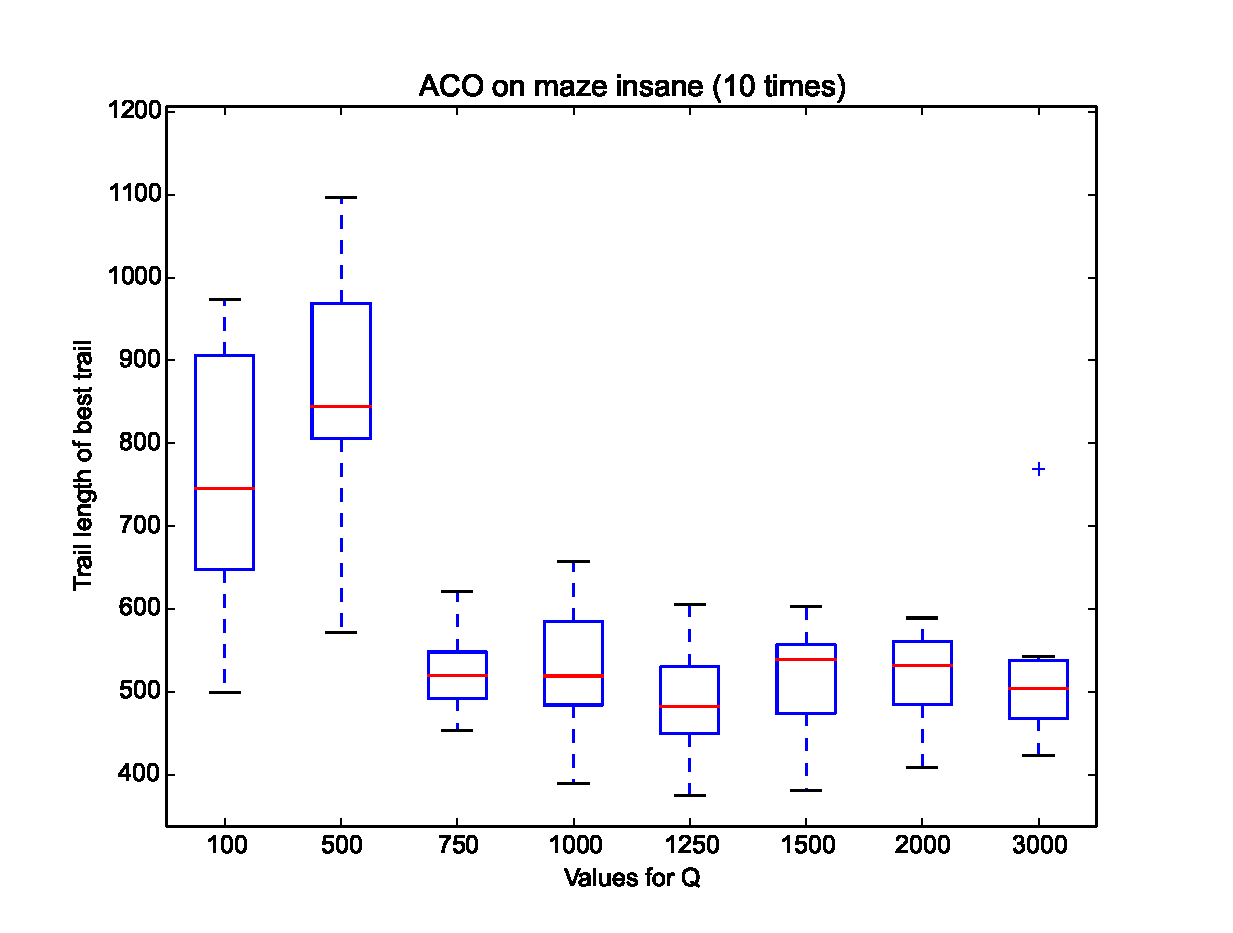
\includegraphics[width=\imwidth]{\impath\immaze/aco-compare-Q-best_trail}
			}\hfill
			\subfloat{
				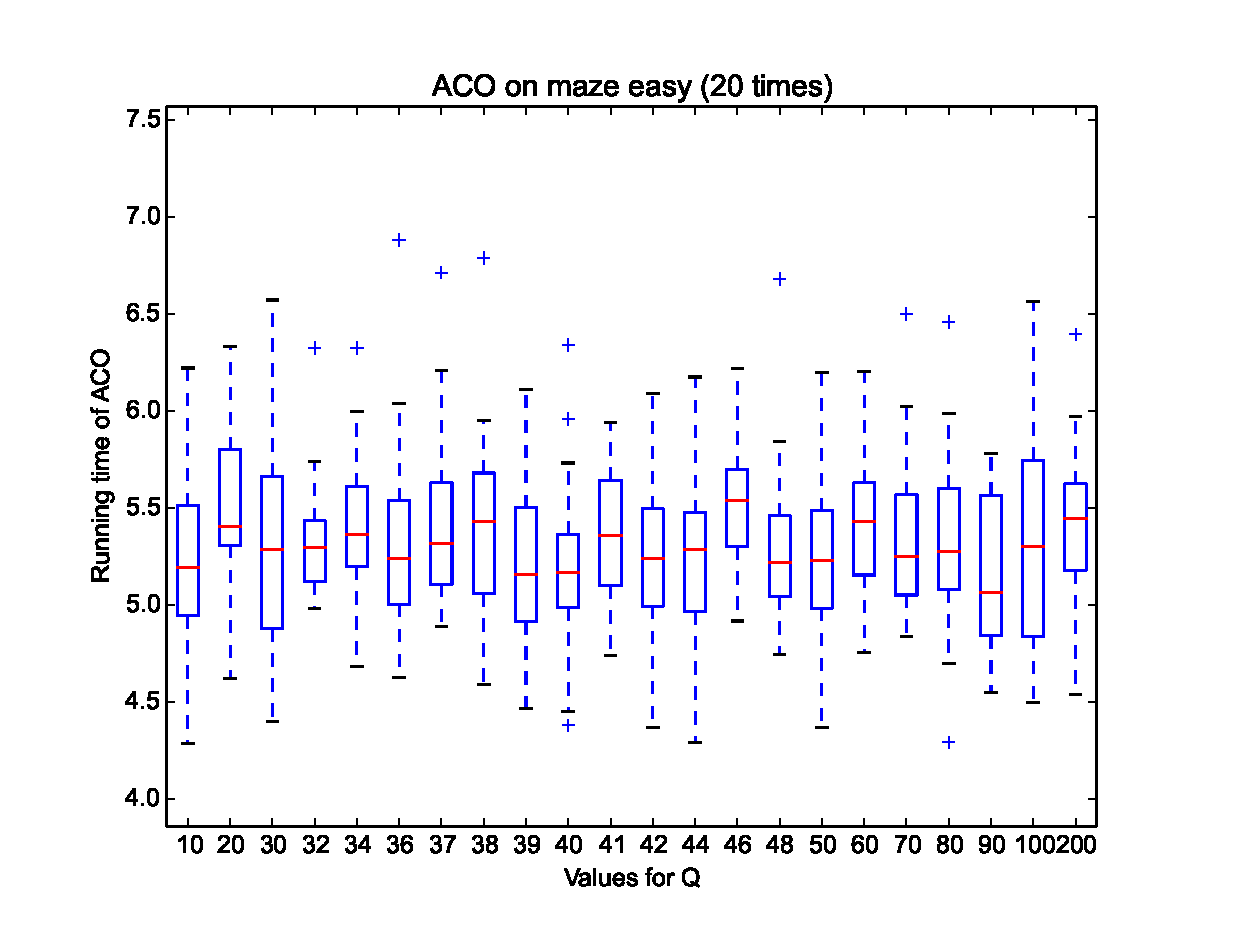
\includegraphics[width=\imwidth]{\impath\immaze/aco-compare-Q-running_time}
			}
		}
		\caption{Variatie van parameter $Q$: lengte van beste trail, running time.}
	\end{figure}

	\begin{figure}[!ht]
		\centering
		\makebox[\textwidth][c]{
			\subfloat{
				\includegraphics[width=\imwidth]{\impath\immaze/aco-compare-ant_count-best_trail}
			}
			\subfloat{
				\includegraphics[width=\imwidth]{\impath\immaze/aco-compare-ant_count-running_time}
			}
		}
		\caption{Variatie van parameter \texttt{ant\_count}: lengte van beste trail, running time.}
	\end{figure}

	\begin{figure}[!ht]
		\centering
		\makebox[\textwidth][c]{
			\subfloat{
				\includegraphics[width=\imwidth]{\impath\immaze/aco-compare-evaporation-best_trail}
			}
			\subfloat{
				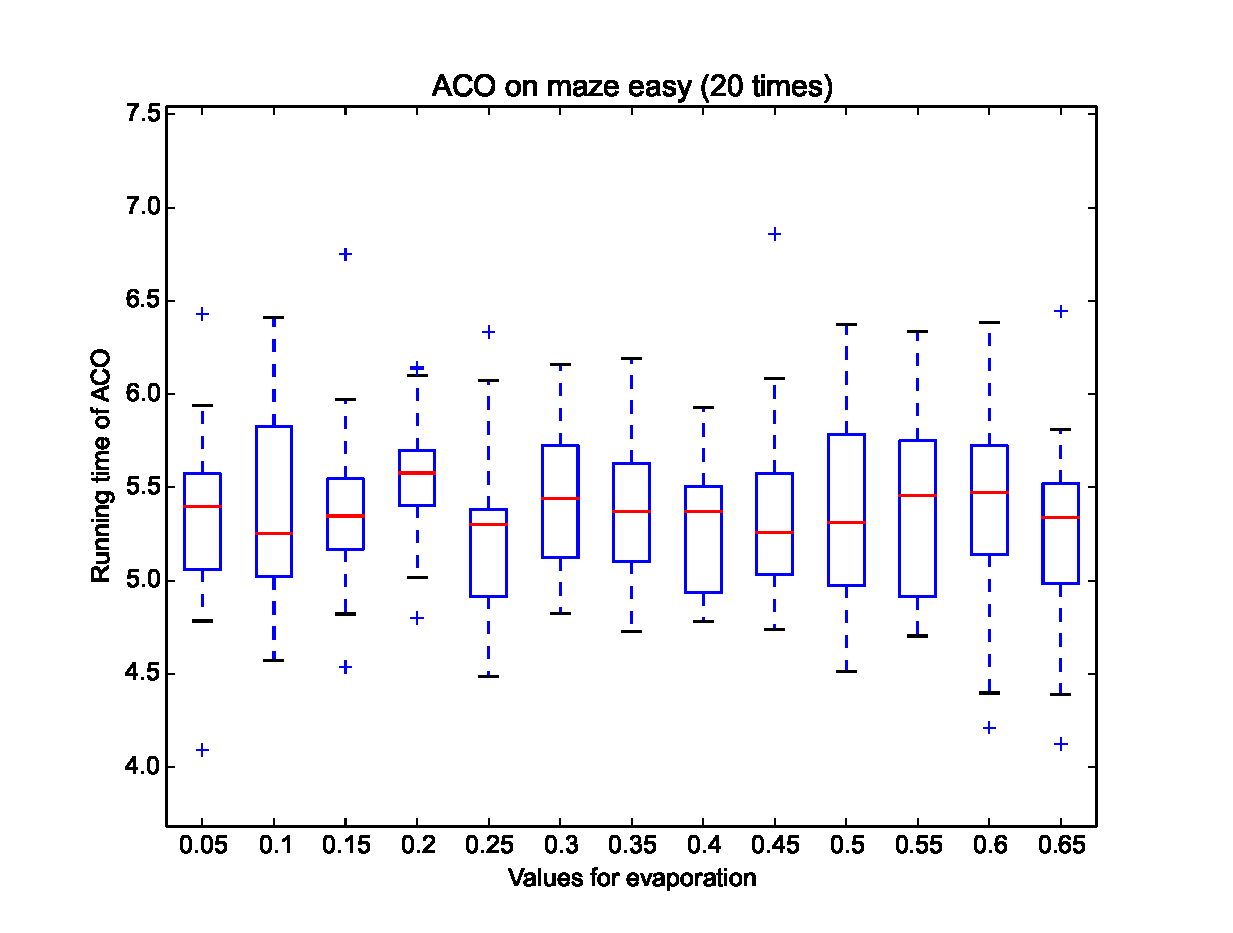
\includegraphics[width=\imwidth]{\impath\immaze/aco-compare-evaporation-running_time}
			}
		}
		\caption{Variatie van parameter \texttt{evaporation}: lengte van beste trail, running time.}
	\end{figure}
	\begin{figure}[!ht]
		\centering
		\makebox[\textwidth][c]{
			\subfloat{
				\includegraphics[width=\imwidth]{\impath\immaze/aco-compare-optimize_ants-best_trail}
			}
			\subfloat{
				\includegraphics[width=\imwidth]{\impath\immaze/aco-compare-optimize_ants-running_time}
			}
		}
		\caption{Variatie van parameter \texttt{optimize\_ants}: lengte van beste trail, running time.}
	\end{figure}
}


\title{TI2736-A Assignment 3: Path finding \& TSP}

\author{
    David Akkerman - 4220390 \\
    Jan Pieter Waagmeester - 1222848 \\
}

\begin{document}
\maketitle

\section*{3.1: Path finding through ACO}
\begin{enumerate}[1.]
    % Make a list of the features you can expect a maze might have. Features that increase the difficulty of ’finding the finish’. Features that will require creative solutions. For example; loops. Name at least 2 other features.
    \item
        \begin{enumerate}[-]
            \item Lange doodlopende straten
            \item Straten met heel veel korte doodlopende zijstraten
            \item Grote open gebieden
        \end{enumerate}


    % 2. Give an equation for the amount of pheromone dropped by the ants. Answer the questions "Why do we drop pheromone?" and "What is the purpose of the algorithm?".
    \item We, of de mieren, laten feromoon vallen om de voordelige paden aan te duiden. Ze laten het feromoon vallen 'op de trugweg', afhankelijk van hoe lang het pad was. Er is een waarde $Q$ die ongeveer de geschatte routelengte is.
    $$\Delta\tau^k = Q \cdot \frac{1}{L^k}$$
    In deze formule staat $\Delta\tau^k$ voor de toe te voegen feromoon afkomstig van mier $k$, $L^k$ de lengte van het pad. Als een pad korter is zullen de afzonderlijke verbindingen van dat pad meer worden versterkt dan wanneer het pad langer was.

    % 3. Give an equation for the evaporation. How much pheromone will vaporise every iteration? This equation should contain variables which you can use to optimize your algorithm. What is the purpose of pheromone evaporation?
    \item Het verdampen van de feromoon is zinnig om niet in een lokaal optimum te blijven hangen. Doordat de waarde in elke cel met een bepaalde verdampingsfactor ($\rho$) afneemt is er kans dat een andere (wellicht betere) route wordt gekozen.
    $$\tau_{ij} = (1 -\rho) \cdot \tau_{ij} + \sum_{k=1}^m \Delta\tau_{ij}^k$$
    \todo {Er moet in ieder geval een vergelijking komen. Wellicht ook met nog wat uitleg en hoe het geoptimaliseerd wordt}

    % 4. Give a short pseudo-code of your ant-algorithm at this stage. If you added any extra functionality to the normal algorithm, please mention and explain them briefly.
    \item Om te beginnen moeten we wat dingen initializeren: een stel mieren en een feromoon-matrix. Vervolgens laten we elke mier een pad zoeken in een matrix waarin de feromoon-waarden in elke cel gelijk zijn.

    Nadat alle mieren het einde gevonden hebben (of getermineerd zijn omdat ze er veel te lang over doen), kiezen we de beste mier uit.
    We laten een bebaald deel $(1 - \alpha) \cdot \tau_{xy}$ verdampen en tellen bij de cellen waar ons beste miertje geweest is een waarde $Q/ |\text{ant}| $ op.

    Daarna gaat het weer opnieuw tot we het aantal iteraties hebben gehad.
    \begin{lstlisting}
ants = [ant0, ant1, ... antN]
pheromone[height][width] = 0.1 # initialize with small value

for i = 0 ... iterations
    foreach ant in ants
        ant.find_naive_solution(halt_after_steps=10000)

    best_ant = select_best(ants)

    pheromone = (1 - alpha) * pheromone

    for p in each best_ant.route
        pheromone (p) += Q / length(best-ant)
\end{lstlisting}
\todo {<-}Ze vragen echt om een ant algorithm, maar hier wordt die als 'vanzelfsprekend' beschouwd en wordt de feromooncode geïllustreerd.
    % 5. Improve the ant algorithm using your own insight. Describe how you improved the standard algorithm; which problems are you tackling and how? Limit yourself to 1 A4 text (excluding aiding figures).
    \item
        We hebben een aantal versnellingsmanieren bedacht en ook bijna allemaal geïmplementeerd.
        \textbf{Doolhofeliminatie} \\
        \begin{description}
            \item[Doodlopende gangen] Als een mier vanaf een bepaalde positie nog maar één kant op kan (terug), zit hij aan het einde van een doodlopende gang. We markeren die plek in de maze dan als muur, zodat er in het vervolg geen mier meer probeert in te lopen.
            \item[Open ruimtes] Hoekjes in een open ruimte kunnen worden weggestreept, als er iets bekend is over de aangrenzende cellen. Als een mier achtereenvolgens een hoekje en daarna twee cellen met voldoende ruimte tegenkomt waarbij de laatste op de diagonaal zit van het hoekje, kan het hoekje worden afgestreept.

            Merk op dat dit bij ons soms mis gaat doordat de mieren afzonderlijk te werk gaan in eigen threads. Het kan dus zijn dat twee of meer mieren er samen voor zorgen dat er een cruciale gang wordt afgesloten. Dit is wel op te lossen, maar gaat voorbij aan deze opdracht.

        \end{description}

        \begin{figure}[!ht]
            \centering
            \includegraphics[width=\textwidth]{images/maze-elimination.png}
            \caption{Voorbeeld van eliminatie van doodlopende stukken. Links na de $1^e$ iteratie, rechts na de $30^e$. Donkerblauwe vlakken zijn door de mieren 'uitgezet'.}
        \end{figure}

        \textbf{Probeer min mogelijk over eigen pad te lopen} \\
        Het heeft niet veel zin om terug te keren waar we al geweest zijn. We geven daarom bij het kiezen van de volgende stap de voorkeur aan de posities waar we nog niet geweest zijn.

        Alleen als het niet anders kan keren we weer terug op of over onze route.

        \textbf{Gebruik het pad van de beste mier over alle iteraties ook bij de feromoon-update} \\
        Door de beste mier in de run van het algoritme tot nu toe te onthouden en elke keer ook te gebruiken voor de update.


        \textbf{Optimalisatie van het gevonden pad} \\
        Vaak is een door een mier gevonden pad niet bijzonder efficient, zeker aan het begin. We kunnen zorgen dat we niet op te veel plekken feromoon neerleggen door voor dat te doen het pad van elke mier nog te optimaliseren:
            \begin{enumerate}[-]
                \item Als de mier langs het einde loopt, direct naar het einde lopen en de rest van de route overslaan.
                \item Als de mier weer langs start loopt het het eerste stuk overslaan.
                \item Als een mier een rondje loopt dat stuk overslaan.
            \end{enumerate}

        \textbf{Andere, niet-geimplementeerde ideeën} \\
        Naast de voorgaande ideeën hebben we nog meer ideeën, waar voor de implementatie helaas de tijd ontbrak:
          \begin{enumerate}[-]
              \item Alle mogelijke stappen hebben lengte $1$, omdat we in een grid werken. We zouden dit kunnen transformeren naar een graaf waarbij we de kruispunten zien als nodes. Dat scheelt een hele hoop mogelijke stappen, en er onstaat variatie in lengte.
          \end{enumerate}


    % 6. Your task is to find a decent set of parameters for each of the grading mazes. You may do so by varying the parameters and subsequently running your algorithm. If your algorithm converges fast to a good route, your parameters are decent. What is ‘converging fast’? Figure that out by varying the parameters.
    % Report your tactic upon how to vary the parameters. Assist your text with graphs showing relationships between the parameters and the speed of convergence. Limit yourself to 1/2 A4 text (excluding aiding graphs - and we like nice informative graphs, so use them!).
    \item We hebben het algoritme laten lopen voor een aantal verschillende waarden van de parameters $Q$, \verb|ant_count|, $\alpha$ and \verb|optimize_ants|. Deze waarden hebben we 20 keer gevarieeerd voor elke doolhof terwijl de andere op een guestimated waarde stonden. Bij elke set van runs meten we drie dingen: run time, in welke iteratie de beste route voor het eerst voorkomt   en de lengte van de beste route.
    Het was even rekenen (1000x easy maze, 760x medium maze, \todo{hard maze}x hard maze), maar levert een hoop ($4 \cdot 3 \cdot 3$) zinnige plaatjes op.

    \begin{description}
        \item[Easy maze] Op grond van deze plaatjes maakt het niet zo veel uit wat we voor parameters gebruiken. Sowieso maakt het allemaal niet zoveel uit, want deze maze is zo klein dat de kortste route altijd wel vrij snel gevonden wordt.
        \item[Medium maze]
        \item[Hard maze]
        \item[Insane maze]
    \end{description}

    Dat brengt ons uiteindelijk bij de volgende waarden:

    \begin{tabular}{l|llll}
                                & easy  & medium    & hard  & insane \\ \hline \hline
        \# iterations           &       &           &       &       \\
        $Q$                     & 38    &           &       &       \\
        \verb|ant_count|        & 50    &           &       &       \\
        $\alpha$                &       &           &       &       \\
        \verb|optimize_ants|    & \verb|True| &     &       &       \\ \hline
        Kortste gevonden route  & 38    & 141       &       &       \\

    \end{tabular}

    \newpage
    % \ACOcompare{}{80mm}

    \todo{medium en hard maze invoegen}

    \todo{Plaatjes maken voor insane maze en eventueel invoegen?}

%     \ACOcompare{medium}{80mm}

    % 7. Using your answer to the previous question, can you say something about the dependency of the parameters on the maze size / complexity? Aim at ≈ 1/4 A4.
    \item



\end{enumerate}

\newpage
\section*{3.2: The Traveling Robot Problem}

\begin{enumerate}[1.]
  \setcounter{enumi}{7}

     % 8. Define the regular TSP problem
    \item Het TSP (Reizende Verkoper Probleem) gaat over een verkoper die een aantal, bijvoorbeeld 20, steden moet bezoeken. Natuurlijk vindt hij het prettig om dit in een zo efficiënt mogelijke volgorde te doen. Het probleem is dat dit erg moeilijk is om uit te rekenen, want het aantal mogelijke volgordes is $ 20! = 2.4\cdot 10^{18}$, wat hij logischerwijs niet allemaal door kan rekenen.

    % 9.  In a classic TSP, all cities (nodes) are singularly connected to all other nodes and relative distances are known and symmetric (a weighted complete graph). How is our problem different?
    \item Het verschil tussen een gebruikelijk TSP en het Reizende Robot Probleem is dat de afstanden tussen de steden van het TSP bekend en duidelijk zijn, terwijl het zich voor ons probleem in een doolhof afspeelt, waarbij verschillende routes tussen twee punten genomen kunnen worden, die niet allemaal zo makkelijk te berekenen zijn.
    \todo{Als je de hele afstandstabel hebt heb je toch in principe hetzelfde als classic TSP?}

    %10.  Why are Computational Intelligence techniques an appropriate tool for solving a TSP?
    \item CI-technieken zijn erg handig om dergelijke problemen op te lossen, doordat ze de rekenkracht van een computer gebruiken, maar op een slimme manier\todo{Herschrijven als: '... op te lossen, doordat ze de rekenkracht van een computer op een slimme manier gebruiken}, waardoor het optimum\todo{Je kan niet garanderen dat je het optimum daadwerkijk vindt toch?} veel sneller gevonden kan worden dan met enkel brute rekenkracht. Door de complexiteit van het doolhof zou het een mens veel langer kosten dan een computer om een goede route te vinden.

    %11.  What do the genes represent and how will you encode your chromosomes
    \item De chromosomen bestaan uit de nummers 1 tot en met 18 en de volgorde waarop deze voorkomen in een chromosoom representeert de volgorde waarop de items opgepakt moeten worden door de robot.
    \todo{Er staat niet letterlijk wat een 'gene' is.}

    %12.  Which fitness function will you use
    \item De fitness functie van het TSP is één gedeeld door de totale afstand die de robot van begin tot eind aflegt als hij alle producten oppakt.

    \todo{Formule erbij doen?}

    %13.  How are parents selected from the population
    \item De ouders worden geselecteerd met een kans die evenredig is met de fitness. Alle oorspronkelijke chromosomen worden gesorteerd op fitness. Vervolgens wordt er een normale kansverdeling gebruikt met verwachtingswaarde 0 en standaardafwijking 75. De absolute waarde hiervan geeft aan welke chromosoom uit de gesorteerde reeks genomen zal worden.
    \todo{Hoe kom je op 75? (Volgens mij was je al van plan daar wat over te gaan schrijven)}

    %14.  The functions of your genetic operations (e.g. cross-over, mutation)
    \item De nieuwe chromosomen worden gecreëerd door zowel cross-over als mutatie toe te passen. Cross-over houdt in dat van een ouderchromosoom een aantal genen gekopiëerd wordt, wat vervolgens de basis is van het kindchromosoom. De missende genen worden aangevuld door deze bij het kind in te plakken in de volgorde waarop ze voorkomen bij een tweede ouderchromosoom.
    \\* Mutatie betekent dat van een ouderchromosoom een willekeurig aantal genen geknipt, omgedraaid en teruggeplakt wordt. Dit wordt gedaan omdat op deze manier stukjes van dicht bij elkaar liggende items niet uit elkaar worden gescheurd, maar alleen in de omgekeerde volgorde bezocht worden, wat kan zorgen voor een verbetering.

    \todo{Doe je altijd een vast aantal, of gebruik je een bepaalde kansverdeling?}

    %15.  How do you prevent points being visited twice?
    \item De oorspronkelijke chromosomen worden zó gecreëerd dat ze precies alle items eenmaal bevatten. De manieren waarop gereproduceerd wordt, zijn zo ontwikkeld dat het niet kan voorkomen dat een kindchromosoom wel tweemaal hetzelfde getal bevat en een ander niet. Bij het mutatie- en cross-overproces wordt namelijk enkel de volgorde van de items veranderd, niet de items zelf.

    %16.  How do you prevent local minima?
    \item Doordat er een normale verdeling gebruikt wordt om de ouders te selecteren, bestaat er altijd een kans dat er een slechter presterend chromosoom gepakt wordt. Dit chromosoom kan in een enkel geval wel betere kinderen geven, waardoor er voorbij een lokaal minimum gegaan kan worden. Om de optimale oplossing te vinden, moet echter een oneindig aantal iteraties plaatsvinden, want je weet niet wanneer de optimale oplossing gevonden gaat worden, maar enkel dát hij ooit gevonden wordt.

    %17.  What is elitism? Have you applied it?
    \item Elitisme houdt in dat een aantal van de fitste chromosomen niet sterven maar ook weer meedoen in de volgende generatie. Op deze manier voorkom je dat er alleen maar minder fitte chromosomen komen. Een gevaar is echter dat er op deze manier te vroeg een lokaal minimum gevonden wordt en niet verder wordt gezocht. Wij hebben elitisme gebruikt in zoverre dat het mogelijk is dat er bij mutatie slechts een rij van één getal wort geïnverteerd, wat geen verandering in het chromosoom aanbrengt, waardoor de ouder dus ongeschonden naar de volgende generatie doorgaat.

\end{enumerate}

\end{document}
